\documentclass[11pt,a4paper]{article}

\usepackage{siunitx}
\usepackage{mhchem}
\usepackage{multirow}

\usepackage[pdftex]{color,graphicx}
\pagestyle{plain}
\usepackage{geometry}
\newgeometry{margin=2.0cm}

\newcommand{\ts}{\textsuperscript}
\newcommand{\ic}{\texttt}
\newcommand{\todo}{TODO: \texttt}

\usepackage[backend=biber,style=authoryear,sorting=nyt,dashed=false]{biblatex}
\renewcommand*{\nameyeardelim}{\addcomma\space}
\addbibresource{references/references.bib} % note the .bib is required

%Wrong spellings!
%parameterization
%parameterizing
%Paracon

\begin{document}

\newgeometry{margin=2.0cm, top=1.8cm}

\begin{center}
    \Large{\textbf{Monitoring Committee Report III}}\\[0.1cm]
    \large{Mark Muetzelfeldt}\\
    \normalsize{9.30am on Monday 19\ts{th} December 2016 in 2U13}\\[0.1cm]		
    \rule{\textwidth}{0.2mm}
    \textbf{Project Title: }Development of scale-awareness in the representation of
    convective cloud systems\\
    \textbf{Monitoring Committee: }Dr Omduth Coceal and  Dr Andrew Turner\\
    \textbf{Supervisors: }Prof. Robert Plant, Prof. Peter Clark, Dr Steve Woolnough \\
    and Dr Alison Stirling (Met Office CASE supervisor)\\
    \rule{\textwidth}{0.2mm}
\end{center}

\section{Project overview}
\label{sec:Project Overview}

To develop a scale-aware parametrization of deep convection, it is necessary to know what the desired effect of the parametrization will be. In a similar vein to \cite{plant2008stochastic}, and more recently \cite{sakradzija2016stochastic} for the shallow cumulus case, the approach taken in this project will be to run high-resolution models to act as the truth, and build the parametrization so that it approximates this truth. In the parametrized case, as the resolution of the model increases, fewer convective clouds will be present in each grid-cell, leading the the breakdown of the quasi-equilibrium assumption of \cite{arakawa1974interaction}. In this case, it is sensible to think of the relationship between the grid scale variables and the parametrized subgrid fluxes as being a statistical one, with the Probability Distribution Function (PDF) of finding a cloud with a given mass flux in a cell being controlled by the grid-mean properties, instead of the subgrid fluxes being deterministically controlled by these properties. In \cite{cohen2006fluctuations}, they found the surprising result that in a Cloud Resolving Model (CRM), convective organization did not seem to have a large effect on the overall statistics of the mass flux of the cloud field, even though it was clearly visible in the location of the clouds. This could be due to a number of factors, e.g. the shear profile that they applied, the limited number of organized cases that they studied or the resolution of the model that they used.

Taking this as a cue, in this project I will look into the effect of shear driven organization in a CRM in a Radiative-Convective Equilibrium (RCE) case. However, I will attempt to produce a more organized cloud field, representative of a squall line for example. Also, the resolution of the model will be higher, at \SI{100}{m} or higher compared with the \SI{2}{km} of the \cite{cohen2006fluctuations} model. The goal will be to reproduce some squall line like features, and then analyse the cloud statistics under this regime. With this in mind, the specific questions that I would like to address are as follows:

\begin{enumerate}
    \item What effect does convective organization have on the overall cloud statistics of idealized RCE models?
    \item How can characterization of this convective organization be used to inform the design of a scale-aware parametrization scheme?
    \item What causes this convective organization?
    \item How can information about fluxes in a high-resolution idealized model be incorporated into a lower-resolution model's parametrization scheme?
\end{enumerate}

Additionally, it would be interesting to see how this deep convection scheme, once it has been developed, behaves in a global simulation, in terms of how it reproduces climatologies and large-scale organization.

The role of resolution will be analysed from the perspective of the convective grey-zone, broadly defined as horizontal resolutions of 10-100 km. Stochastic schemes lend themselves well to being scale-aware as there is a natural way of increasing the grid-scale variability as the resolution of the model increases \parencite{plant2008stochastic, sakradzija2016stochastic}. Parametrized models can be run in this range of resolutions, and their output can be compared to the coarse-grained output from the CRM. This will allow for the validation of the parametrization scheme, as well as a characterization of its shortcomings. It will also act as a test-bed for making changes to the parametrization scheme to represent the effects of organization in this scheme. 

% Momentum fluxes.

% LESs being fed into p13n schemes?

\resetgeometry

\subsection{Background reading}

\subsubsection{High-resolution modelling}
% High res modelling.
% Efstathiou et al.
% A key part of my project will be running the idealized high resolution model. Given that the model that I am using, the iUM (idealised UM), is a new model which has not been used by all that many people so far, it is necessary for me to be sure that I have configured it correctly. This has involved learning more about the various schemes which it employs, such as the boundary layer scheme and the turbulence scheme, and finding out which particular science settings I should be using. As a concrete example, I had been using the blended boundary layer scheme \parencite{boutle2014seamless}. From interactions with Adrian Lock at the Met Office, I was advised that this scheme might not be appropriate for high-resolution models, where even though it can reproduce the adiabatic profiles in the boundary layer, it underestimates turbulence \parencite{efstathiou2016grey}.  

The work done in 2006 on CRMs \parencite{craig2006fluctuations, cohen2006fluctuations} will serve as inspiration for the high-resolution modelling I will perform. They first provide a theoretical framework for calculating the PDF of a given area of interest having a particular mass flux, which is given by:

\begin{equation}
    p(M) = \sqrt{\frac{\langle N \rangle}{\langle m \rangle}} e^{-\langle N \rangle} M^{-\frac{1}{2}} e^{\frac{-M}{\langle m \rangle}} I_1\left(2 \sqrt{\frac{\langle N \rangle}{\langle m \rangle} M}\right).
    \label{eqn:pdf_mass_flux}
\end{equation}

Here the angle brackets denote an ensemble mean. $p(M)$ is the probability of finding an area of interest with a given mass flux, $M$, $\langle M \rangle$ is the mean convective mass flux over the area of interest at a given height, $\langle m \rangle$ is the mean mass flux per cloud. $\langle N \rangle = \frac{\langle M \rangle}{\langle m \rangle}$ is the mean number of clouds in the area of interest. $I_1(x)$ is the modified Bessel function of order 1. Whilst the form of this PDF may not be immediately obvious, its shape is similar to a Poisson distribution (see Fig. \ref{fig:pdf_mass_flux} (b)), and it becomes more Gaussian as $\langle N \rangle$ increases in accordance with the central limit theorem (see Fig. \ref{fig:pdf_mass_flux} (a)).

\begin{figure}[hbp!]
    \centering
    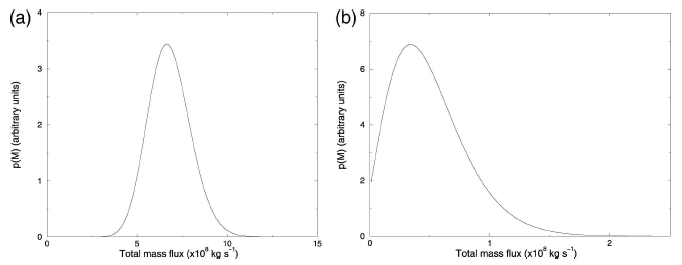
\includegraphics[width=400px]{figures/CraigAndCohenFig2}
    \caption{Theoretical PDF of total mass flux, $p(M)$, for: (a) $\langle N \rangle = 68$; (b) $\langle N \rangle = 5$; $\langle m \rangle = 10^7$ \SI{}{kg.s^{-1}} in both cases. Taken from \cite{cohen2006fluctuations}, their Fig. 2.}
    \label{fig:pdf_mass_flux}
\end{figure}

In their second paper they go on to match these theoretical findings to output from a CRM run at \SI{2}{km} resolution \parencite{cohen2006fluctuations}. They compare an RCE case forced by prescribed cooling in the range \SI{2}{K.dy^{-1}} to \SI{16}{K.dy^{-1}}, with the limits representative of radiative cooling over oceans and an exaggerated form of dynamically forced ascent respectively. They find that the form of Eq. \ref{eqn:pdf_mass_flux} fits well with the distribution derived from the model data provided the values of $\langle N \rangle$ and $\langle m \rangle$ are fitted to this distribution (their Fig. 3). If, however, $\langle N \rangle$ and $\langle m \rangle$  are diagnosed from the model, then Eq. \ref{eqn:pdf_mass_flux} overestimates the variance of the distribution by between 10 and 20 \%, depending on whether the size of individual clouds is taken into account. Additionally, they go on to look at an organized case where wind shear is applied across the domain, generating mesoscale arcs. They find that these cases can still be described by their model. In fact the greater variance shown by the organized case brings it closer to their predicted model, although this is likely due to the organization acting ``to offset the reduced variance seen in the unsheared simulations''.


\subsubsection{Parametrization schemes}
In previous Monitoring Committee reports I have picked one or two parametrization schemes and looked into them in some detail. Now I am trying to take a step back and to find the general features that schemes have in common, e.g. the mass flux paradigm that is common to many schemes. To do this, I have been reading review articles such as the one by \cite{arakawa2004cumulus}, which provides a good history of parametrization schemes and emphasizes the similarity of their outcomes, even when they have been formulated in quite different ways. 

The chapter on ``Convective parameterizations'' in the book by \cite{stensrud2009parameterization} tries to classify the various schemes by certain criteria. He uses the criterion of ``deep-layer control'' as one way of distinguishing between the various schemes, as well as talking about triggering and closures of the schemes. I am currently in the process of drafting a literature review of these schemes, which will serve both as a useful document of how these schemes work and how they are related to each other, and as a basis for a large part of my literature review for my thesis.

% Parametrization overviews.
% Arakawa 2004
% Stensrud
% Davies thesis
% Daleu thesis
% Pan and Randall
% Kain Fritsch

% Stochastic parametrizations.

\subsubsection{Moisture conservation in semi-lagrangian models}
\label{sec:MC_in_SL}
The issues described below in Sections \ref{sec:modelling} and \ref{sec:MC_sensitivity} with moisture non-conservation have necessitated that I understand more about Moisture Conservation (MC) schemes in the UM. For current purposes, the three schemes that are relevant are the Priestley scheme \parencite{priestley1993quasi}, the All Dancing All Singing (ADAS) scheme \parencite{zerroukat2010simple} and the Optimized Conservative Filter (OCF) scheme \parencite{zerroukat2015monotonic}. %(other schemes are relevant when considering nested Limited Area Models and flow across their boundaries). 
These schemes perform roughly the same job, and without going into detail they are used to ensure MC in the UM by diagnosing any non-conservation at each timestep and optimally adding or removing moisture from the model to make up the imbalance.
% Moisture conservation.
% a few...
% eternal fountain.

\subsubsection{Additional reading}
I have started reading into shear-driven organization, to get a sense of how to develop a range of shear profiles for the purpose of analysing the effects of shear in numerical simulations. I have also done some preliminary reading into how momentum fluxes can be included in a parametrization scheme.


\section{Completed work}

\subsection{Modelling}
\label{sec:modelling}
% Link back to MC2 future work.
In the ``Future work'' section of my previous Monitoring Committee Report, I wrote first that I would start with iUM vn10.4 and use this at a \SI{1}{km} grid length to serve as a basis for my future modelling. I have kept up-to-date with developments to this branch, updating to vn10.5 (and shortly to vn10.6) following Chris Smith's work at the Met Office. This has involved making numerous small changes to the model's science settings to work towards getting the model properly configured, e.g. checking settings for input SST are set correctly or the appropriate boundary layer scheme is in use. I have run a range of analyses on the output, with some of these presented below. One particular finding has dominated all the others though: the non-conservation of moisture in the model. The semi-lagrangian scheme is not conservative, and the magnitude of this non-conservation in the iUM has caused some consternation among my supervisors and me, and finding out why it is happening and what steps can be taken to improve it has taken precedence over other aspects of my work. This non-conservation is larger in magnitude than similar results found recently by Chris Holloway using a similar setup with vn7.5, or by previous work by Steve Woolnough in 2009.

\subsection{MC sensitivity}
\label{sec:MC_sensitivity}
% Sensitivity report.
The main portion of this work involved performing sensitivity tests to various aspects of the model settings. I ran experiments with MC on as a control on a 64$\times$64 \SI{}{km^2} domain with a \SI{60}{s} timestep, and relaxation back to a $u$ wind of \SI{-5}{m.s^{-1}}, and MC off with a variety of different settings: \SI{60}{s}, \SI{30}{s}, \SI{15}{s}, no prognostic graupel and on a 256$\times$256 \SI{}{km^2} domain. The findings were that with MC on, the precipitation matched the LHF, as it should, but the precipitation was greater than 3 times too large with MC off, and was insensitive to the different settings changed above. This is shown for MC on and off, with otherwise identical settings as the control run, in Fig. \ref{fig:MC_on_off}, demonstrating that the precipitation balances the evaporation with MC on, and the precipitation is approximately 3 times too large with MC off. These were all performed with a vertical level set of 98 levels, based on the LEM level set. The first level is \SI{63}{m} above the ground, which may have led to the under-resolution of the vertical superadiabat, and it was believed may have contributed to the moisture non-conservation. However, running with the standard UM level set of 70 levels, where the first level is \SI{5}{m} above the surface, produced almost identical results, indicating that the vertical resolution was not the cause of the moisture non-conservation. 

\begin{figure}[htp!]
    \centering
    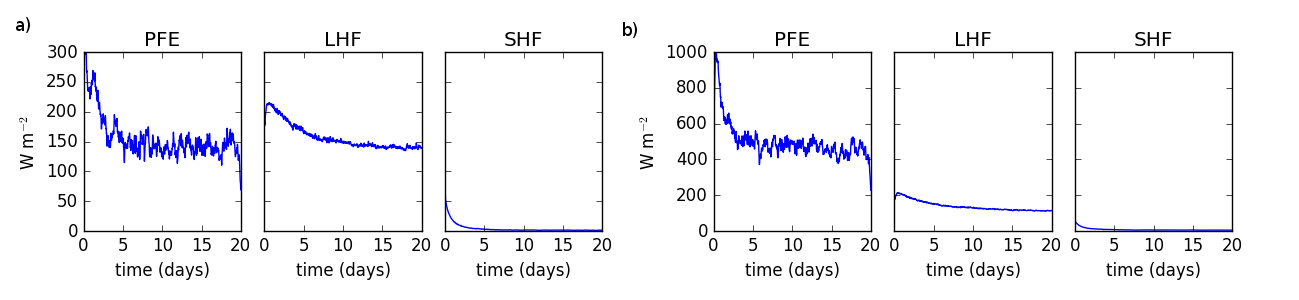
\includegraphics[width=450px]{figures/surf_ts_plots_MC_on_off}
    \caption{Comparison of Precipitation Flux Equivalent (PFE), Latent and Sensible Heat Flux (LHF and SHF) for a) MC on and b) MC off. Both runs are done on a 64$\times$64 \SI{}{km^2} domain with a \SI{60}{s} timestep. An averaging window of \SI{12}{hrs} is used for the PFE, with a noticeable artefact of this window visible at the end of the \SI{20}{day} runs.}
    \label{fig:MC_on_off}
\end{figure}

As a recent update on this work, a critical bug in the iUM has been found. This bug was found just before the ParaCon plenary (see Section \ref{sec:paracon_plenary}), and initiated a fair amount of discussion from those attending. The Smagorinsky code was found to be diffusive only in the $x$ direction, and not in the $y$ direction, leading to a collapse of the convection into 1D structures in the $x$ direction. An example of this is shown in Fig. \ref{fig:precip_MC_on_off}. At the time, I believed that this behaviour was caused by the model dynamics acting as it should combined with the relaxation back to a mean wind across the domain, but in retrospect it appears that this is in fact a manifestation of the bug with the Smagorinsky code. Now that this bug has been identified, a fix has also been added to the vn10.6 iUM branch. Testing that this fix works for me will be a priority.

\begin{figure}[htp!]
    \centering
    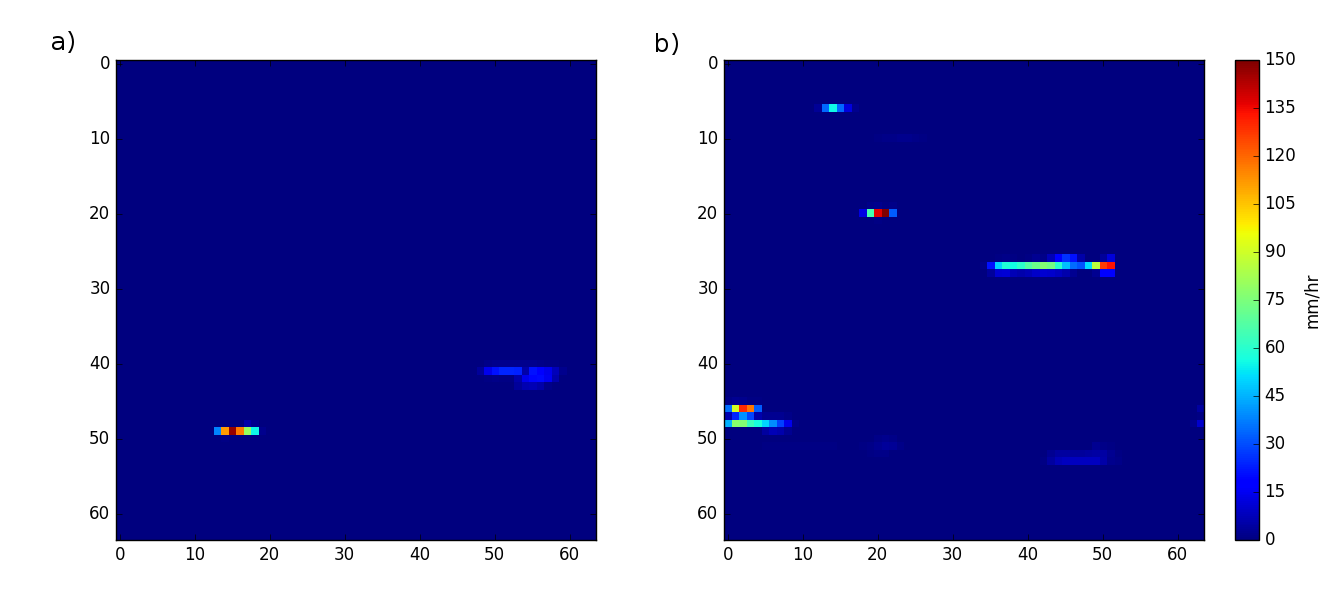
\includegraphics[width=380px]{figures/surf_precip_MC_on_off}
    \caption{Surface precipitation shown after \SI{20}{days} for a) MC on and b) MC off. The model is relaxed back to a $u$ wind of \SI{-5}{m.s^{-1}}. The greater precipitation in the MC off experiment is evident, as is the collapsing of the convection into 1D structures in both cases. }
    \label{fig:precip_MC_on_off}
\end{figure}

Investigating this MC issue has taken up a lot of my time. It has, however, been instructive for several reasons. I have learnt about the MC schemes in the UM, how to make changes to the model, how to perform a reasonably wide range of analysis, who to communicate with at the Met Office when things go wrong with the iUM and how to organize my experiments. Beyond this, it is necessary work for me to have trust in the high-resolution model's output. Given that I am using this output as the truth, this is quite important. 


\subsection{Other analysis}
% Other analysis
% I have been using the output I have to work on further analysis. Investigating the MC issue required me to analyse domain mean quantities of e.g. specific moisture vapour, $q$, cloud liquid water, $qcl$, and other hydrometeors. On comparison of the resulting 2D fields that I got from performing the mass weighted vertically integral of these quantities with the 2D fields available in the UM diagnostics, I noticed a discrepancy which I believe is due to an inconsistency of the way that these fields are calculated in the UM. 

I have performed some rudimentary cloud-cell tracking. This works by using the mass weighted vertical integral of $qcl$ as measure of where the clouds are, with an arbitrary threshold value being picked to perform the cell tracking. Contiguous ``blobs'' of clouds with a value above these thresholds are detected, and then tracked from one timestep to the next by looking at overlaps. This allowed me to generate animations of vertical profiles of the moisture variables for the MC on and off experiments. This code, or similar code obtained from either Juwon Kim and Thorwald Stein or another group, will let me build more detailed cloud lifetime statistics in the future. 

% omnium
% Doing this analysis I have tried to be rigorous in recording the runs I have done and making sure that the work that I do is reproducible. I am keeping a record of all the runs I am doing and storing the output on the ARCHER RDF, since the end of August I have done 38 successful runs. For results analysis, I am using a set of tools called omnium, which I have written to allow me to theoretically reproduce any figures or data I need from the iUM output. It also has the capability to show 3D fields in realtime, which allows for e.g. visualization of clouds to pick interesting clouds for further analysis.

\section{Future work}
% As set out in my PhD Plan...

\subsection{PhD plan}
It is easy to get lost in the day-to-day details of what has to be done next. To make it easier to keep the big picture in mind, I have produced a PhD planning document that breaks the work down into manageable chunks, with defined deliverables and timelines. This is a ``living document'' that I will update over the course of my PhD, to reflect the incremental changes that are necessary as my PhD progresses. In broad terms, Phase 0 is where I am now, which involves making sure that the model is behaving as it should do, and Phase 1 will form the next part of my work, investigating cloud statistics and organization in high-resolution models, which will be described in detail in Section \ref{sec:high_res_modelling}.

\subsection{Moisture non-conservation}

The first thing I will do is to see whether the fix for the critical bug discussed in Section \ref{sec:MC_sensitivity} works as intended. This may well fix the MC issues I have seen entirely, or it may drastically reduce the magnitude of the problem. If there is some residual moisture non-conservation, I may still want to run with an MC scheme, such as the OCF scheme currently being used. This will mean that I should still put some work in to determining exactly how much moisture the scheme is removing.

To do this, I will finish off my investigation into the moisture non-conservation issue. This will involve adding in a 3D diagnostic to determine how much moisture is being removed by the MC scheme. I have been in touch with Mohamed Zerroukat at the Met Office, who implemented most of the MC schemes in the UM, to get details on how to do this. He has suggested a suitable modification to the code to add this in, and this should allow me to create a diagnostic for this field. With this diagnostic, I will be able to look at where the moisture is being added or removed, and what the magnitude of the amount of water that has to be added or removed is. I am mindful that this has taken up a lot of my time in the last 6 months, and that I need to move on from this early in 2017.

\subsection{High-resolution modelling}
\label{sec:high_res_modelling}
Following this, I will begin work on the high-resolution modelling, deriving cloud statistics and information about fluxes of energy, moisture and momentum, as set out in Phase 1 of my PhD plan. I will perform experiments with and without vertical shear across the domain, to characterize the change in cloud statistics when organization is present or absent. This will form a self-contained piece of work, which will have content that will fit nicely into one chapter of my thesis, and will also form a substantive piece of that I will be able to present at the next monitoring committee.

In the longer term, I will start using the results from the high-resolution modelling to inform the design of a stochastic scale-aware parametrization that is based on the \cite{plant2008stochastic} scheme, with the novel addition of either or both of momentum fluxes or large-scale organization depending on the preliminary results of the analysis.

\section{Training record}

\subsection{ParaCon plenary in Leeds}
\label{sec:paracon_plenary}
The second ParaCon (Parametrized Convection) plenary was held in Leeds on the 7\ts{th}-8\ts{th} of December. This was a chance for the five main projects to get together and discuss progress as well as the potential for collaboration. One key part of the project is the generation of high-resolution output that will be used by a few of the different projects for a variety of different purposes, such as the statistical analysis of cloud fields and the analysis of fluxes of heat, moisture as well as potentially higher order quantities. One of the initial test cases that will be run is an RCE experiment, using the iUM and MONC (Met Office NERC Cloud Model). As such, there is a large degree of overlap between these runs and the runs I will need for my PhD, and the potential for me to use some of these output data as part of my studies and analyses. These runs could potentially use very large domains and high-resolutions, meaning that they could be invaluable for analysing the upscale organization of convection.

At the conference I presented printed slides of my work into moisture non-conservation (in place of a poster). The talks I attended provided an overview of the work of the various groups, some were useful in terms of finding out what is going with the iUM/MONC, and others gave me references to interesting papers that I would like to follow up on. The discussion sessions offered a good chance to interact with a variety of people on relevant topics for me, such as the link between convection and upscale organization and what diagnostics will be required from the high-resolution models. It was also a good chance to build connections with other PhD students and Post-Docs from other institutions.


\label{sec:Training record}
\subsection{Transferable skills}
% RRDP.
% Demonstrating. + invigilating
I have been demonstrating in Hilary Weller's Numerical Modelling practical classes. This has given me experience of helping out students with their code problems, trying to quickly diagnose code issues from looking at a plot that does not show what it is meant to, or by scanning code on a screen. % This has also involved answering their questions on anything from the use of modulo arithmetic, how to structure code or how a particular numerical scheme should behave. I enjoy helping out in these classes, trying to tailor my answers to match the way that a particular student approaches a given problem, and following up with teaser questions to get the students thinking about something else were appropriate.

I have continued my responsibilities as a 2\ts{nd} year representative for the Post Graduate Research forum, providing a perspective from a mature student's point of view. I have helped to edit the PhD blog, The Social Metwork, which gives me practice reading over text in detail looking for mistakes and inaccuracies, as well as helping me to get a feel for what works well as blog content. 

As part of the Walker Institute's Climate Action Studio initiative, I was actively involved in the COP22 Marrakech conference.  We attended some of the side-events via the live-streamed youtube channels, allowing us to virtually experience the discussions that were taking place there, as well as asking questions from our computers and also remotely interviewing some of the attendees by Skype. % We were given the opportunity to interview some of the speakers and other attendees of the conference via Skype as well. Four PhD students gathered round a computer in an office in the Walker Institute, and two other PhD students who were in Marrakech found interviewees from the conference for us to interview. We spoke to Teresa Anderson from ActionAid, \todo{other ppl}, taking it in turns to lead the interview with other students chiming in with relevant questions. It was a great way for us to interact with attendees, finding out their thoughts on topics such as what they would like from scientists, how we can communicate our work, and what they thought of the recently elected Trump. 
% It also reminded us that what we are working towards as scientists is vitally important in terms of shaping the debate around climate change, and gave us the chance to think about how to talk about our PhDs in a way that is more easily comprehensible to a wider audience. For example, if I say I am looking at stochastic parametrization of deep cumulus convection schemes in the grey-zone, I will draw blank looks from everyone that I meet. If I say I am working to improve the representation of clouds in climate models, then people will likely be able to make sense of this.

% Speaking in Mesoscale group.
In November I talked in Mesoscale group for 50 minutes on the work I have been doing analysing the iUM's output. I highlighted some aspects of the moisture non-conservation issues that I have come across, and gave some information about why this happens, and what can be done to improve the situation. % At the end, I gave a brief demonstration of the 3D viewing software I have developed for viewing the iUM's output. 
Speaking in front of people is not something that I am fond of, so this was a good chance to practise it in a benign environment which will make it easier in the future.

\printbibliography[title={References}]

\newpage
\section*{Appendix}

\subsection*{Training record}
\subsubsection*{Year 1}

\begin{itemize}
  \item RRDP: Intermediate/Advanced \LaTeX\ (4/11/2015)
  \item RRDP: You and your supervisor (11/11/2015)
  \item RRDP: Quality assurance in research (18/11/2015)
  \item RRDP (equivalent): UM Training (16-18/12/2015)
  \item RRDP (equivalent): Preparing to teach: Introduction to teaching and Learning (26/1/2016)
  \item Preparing to teach: Marking and feedback (26/1/2016)
  \item Preparing to teach: Laboratory demonstrating and leading small groups (27/1/2016)
  \item MONC Training course (9-10/2/2016)
  \item RRDP (equivalent): Fairbrother Lecture ``A slippery situation: melting ice in Antarctica'' (4/5/2016)
  \item ECMWF Parametrization of subgrid physical processes (16-20/5/2016)
\end{itemize}

\subsubsection*{Year 2}

\begin{itemize}
  \item RRDP: Managing your research project (17/11/2016)
  \item RRDP (booked): How to write a thesis (24/1/2017)
  \item RRDP (booked): Presentation skills (7/3/2017)
  \item RRDP (booked): How to write a paper (8/3/2017)
\end{itemize}

\subsection*{Talks and conferences}

\begin{itemize}
  \item Climate Change 2013: The physical science basis. Institute of Physics (2/2014)
  \item Dame Julia Slingo: Taking the planet into uncharted territory: What climate models can tell us about the future (9/2014)
  \item SCENARIO NERC DTP Conference (9/6/2015)
  \item Climate Change in the run-up to the Paris conference: what has Physics got to say? (6/11/2015)
  \item RMetS talk: The risk and vulnerability of Europe to severe convective storms (6/4/2016)
  \item ParaCon Plenary 1 in Reading (27-28/6/2016)
  \item RMetS debate: What will make the public and politicians take climate change more seriously? (5/10/2016)
  \item RMetS talks: Come Rain or Come Shine (19/10/2016)
  \item COP22 Marrakech: Remote participation (11/11/2016)
  \item ParaCon plenary 2 in Leeds (6-7/12/2016)
  \item RMetS talks: Chaos and Confidence in Weather Forecasting (14/12/2016)
\end{itemize}

\end{document}